
% The \section{} command formats and sets the title of this
% section. We'll deal with labels later.
\section{Introduction}
\label{sec:intro}

Rock-Paper-Scissors (RPS) is a simple game played between two opponents.  Each round, players make simultaneous moves, each employing one of three hand positions, representing three different actions: rock, paper, or scissors.  The goal for each player is to choose the action that will defeat the opponent's move subject to the rules of the game: rock defeats scissors, scissors defeat paper, and paper defeats rock.  Figure~\ref{fig:rps} illustrates the cyclic rules for winning a round.

Succeeding in RPS is highly dependent on chance, as is obvious from a cyclic game with a small number of moves of equivalent value.  To avoid indistinguishable wins, algorithms are compared by their competitive performance over a large number of rounds -- for the purposes of this paper, $10000$.

The Nash equilibrium is the balanced equilibrium of moves if both players play optimally, knowing the other player's strategy, and will not benefit from changing their strategy. For Rock-Paper-Scissors, the Nash equilibrium is a probabilistic balanced distribution of each of the three moves \cite{noregrets}.  The Nash equilibrium will, on average, tie every strategy.  Therefore, it is to our advantage to use a strategy that will optimize its play against non-random players.  

\begin{figure}[ht]
	\centering
	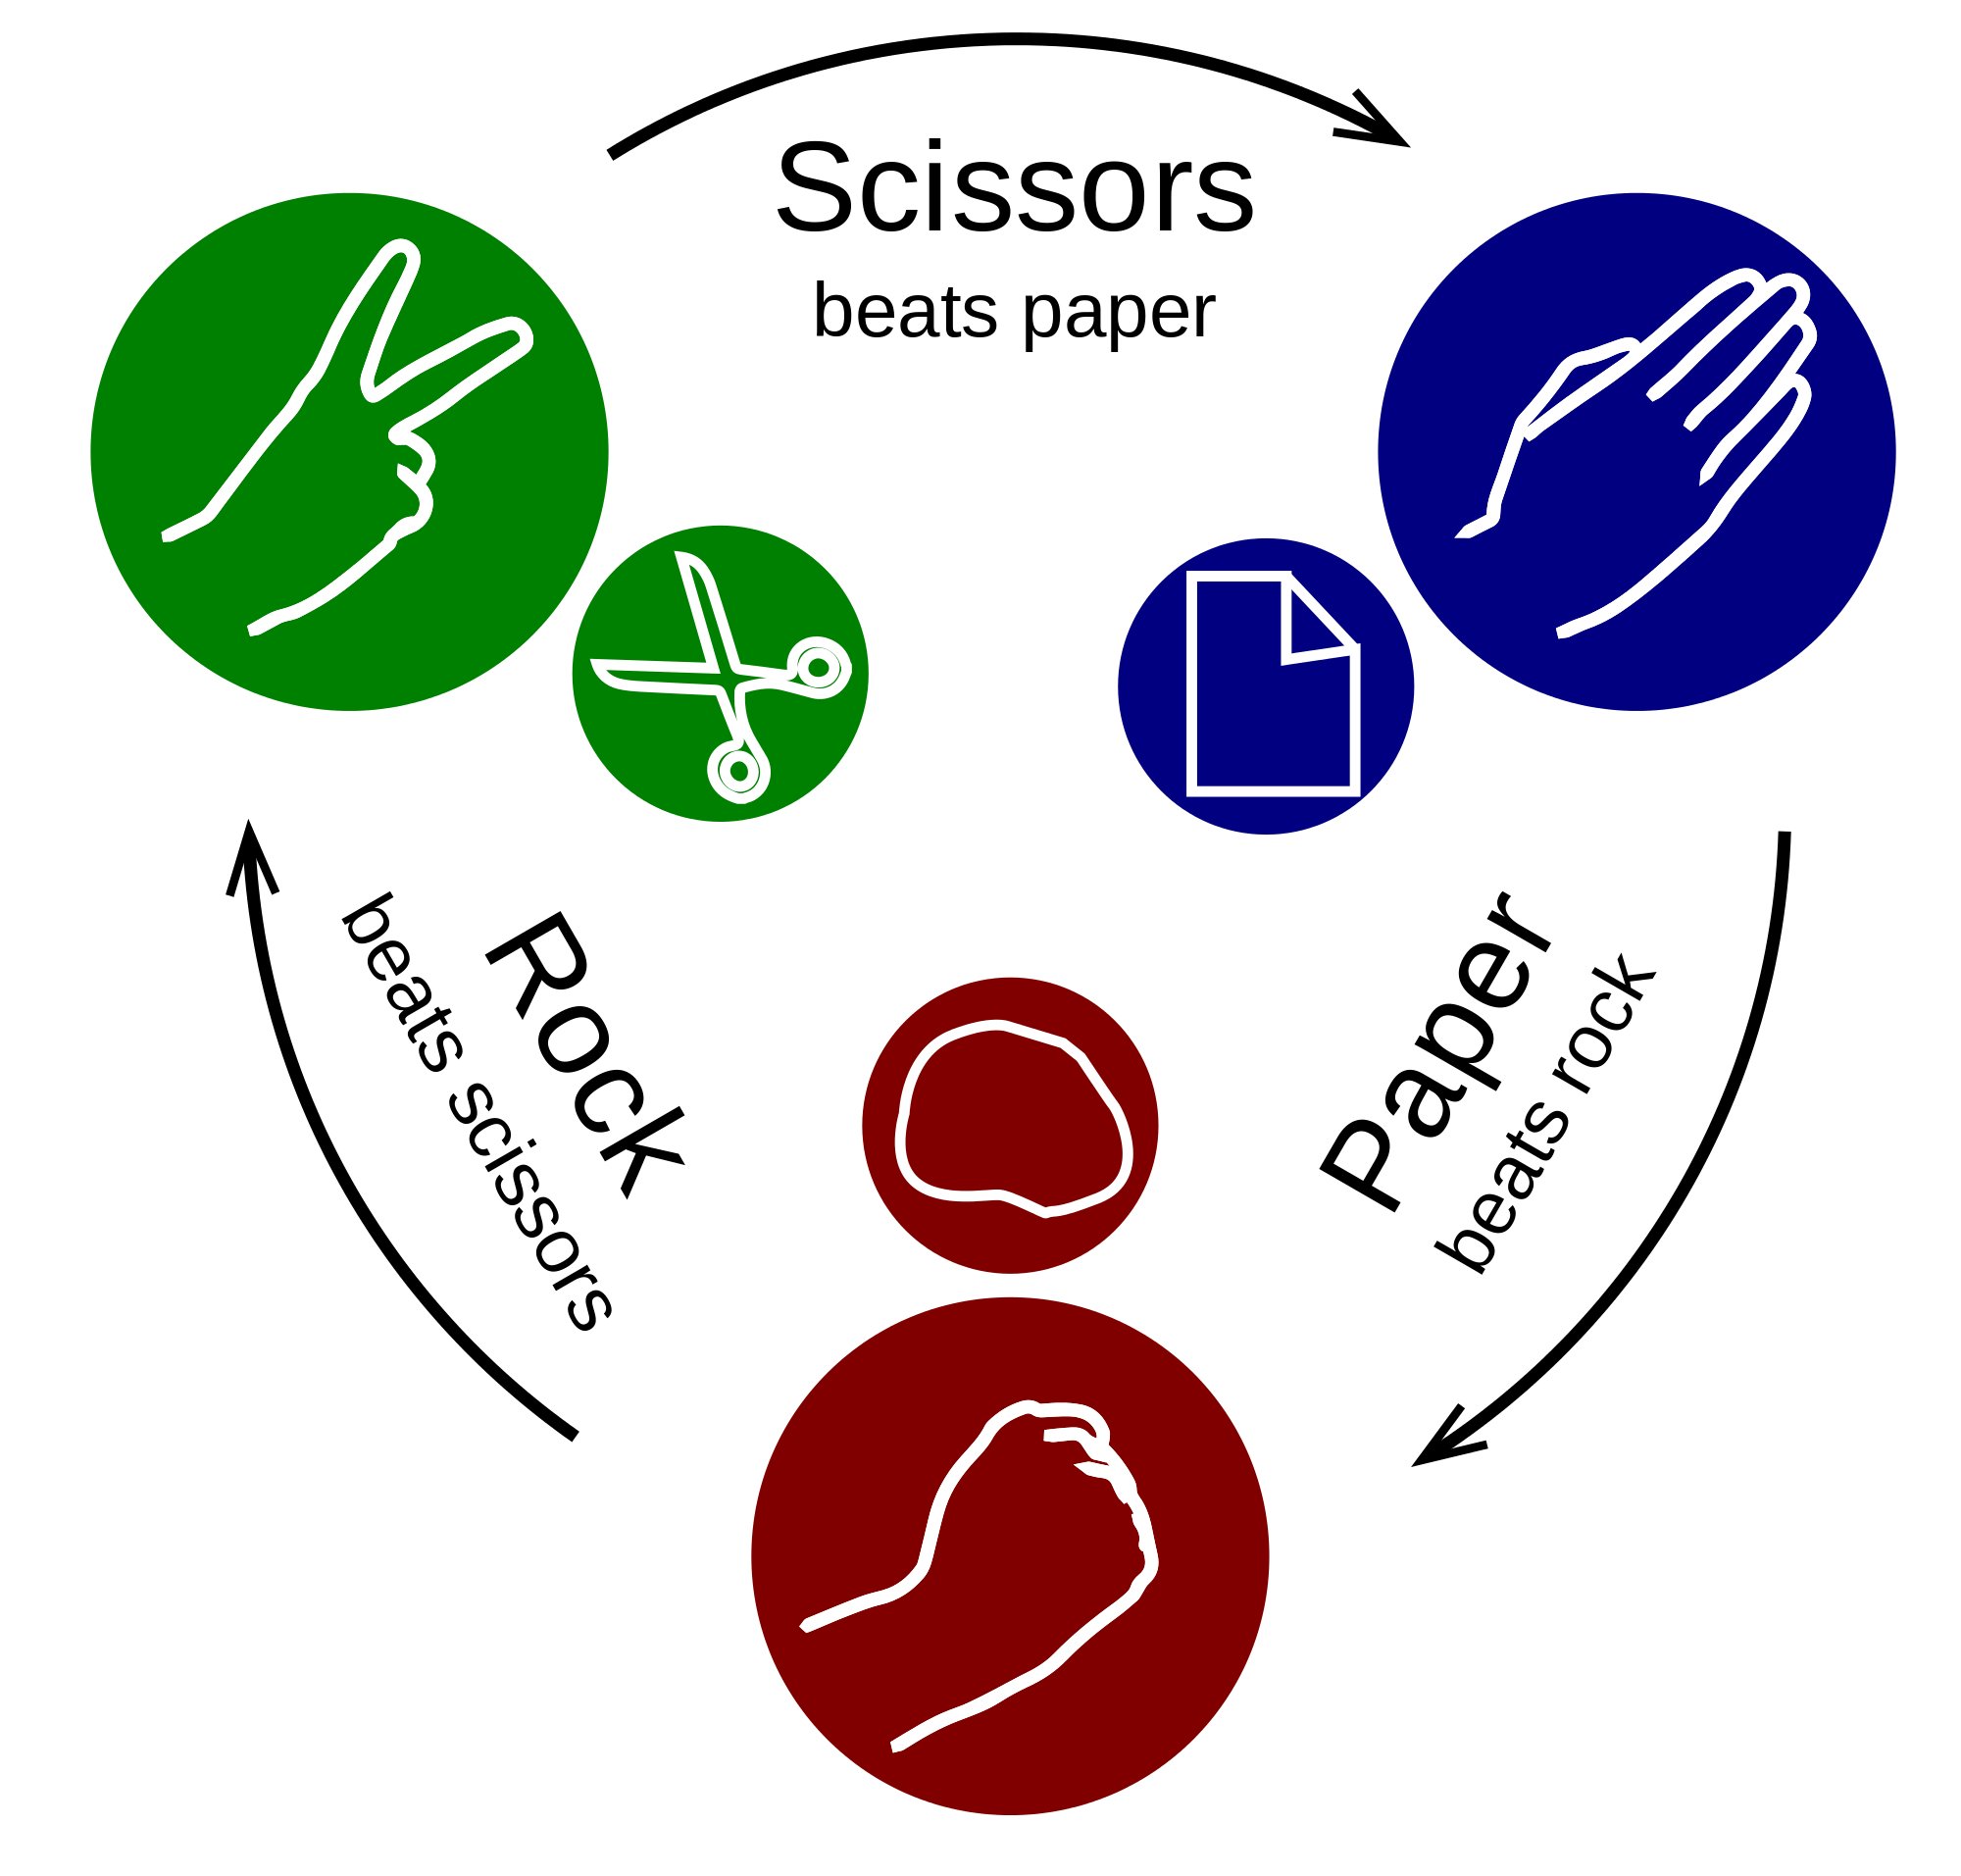
\includegraphics[width=0.47\textwidth]{figs/rps.png}
	\caption{Rock-Paper-Scissors has a circular set of rules \cite{fig:rps}.}
	\label{fig:rps}
\end{figure}

To improve performance against non-Nash algorithms, we can consider choices of moves in terms of regret.  Regret, in general, is the response to learning that, for a past decision, another choice would have resulted in a better outcome.  In application to games, regret can be applied in hindsight to evaluate the benefit of having made a different choice of action.  By determining the regret associated with past moves, a player can anticipate the regret associated with a given upcoming move.  In order to win, players naturally intend to minimize regret.  Regret minimization algorithms use this approach to choose the optimal choice at each step in order to anticipate, and therefore beat, the opponent's move.

In this paper, we describe the creation of a regret-minimization algorithm to compete against computational opponents in Rock-Paper-Scissors.

%In this section, you should introduce the reader to the problem you
%are attempting to solve. For example, for the first project: describe
%the $15$-puzzle, and why it's interesting as an A.I. problem. You
%should also cite and briefly describe other related papers that have
%tackled this problem in the past --- things that came up during the
%course of your research. In the AAAI style, citations look like
%\cite{aima} (see the comments in the source file \texttt{intro.tex} to
%see how this citation was produced). Conclude by summarizing how the
%remainder of the paper is organized. \\

%Overall, the aim in this section is context-setting: what is the
%big-picture surrounding the problem you are tackling here?

